\documentclass[11pt,a4paper]{article}
\usepackage[UTF8]{ctex}
\usepackage{geometry}
\usepackage{graphicx}
\usepackage{xcolor}
\usepackage{hyperref}
\usepackage{fancyhdr}
\usepackage{titlesec}
\usepackage{listings}
\usepackage{booktabs}
\usepackage{caption}

\geometry{left=2.5cm,right=2.5cm,top=2.5cm,bottom=2.5cm}
\hypersetup{colorlinks=true,linkcolor=blue,urlcolor=blue}

\titleformat{\section}{\large\bfseries\color{blue!80!black}}{}{0em}{}[\vspace{0.3em}\hrule]
\titleformat{\subsection}{\normalsize\bfseries}{}{0em}{}

\pagestyle{fancy}
\fancyhf{}
\fancyhead[L]{\small 工单系统 · 追加功能使用手册}
\fancyhead[R]{\small v1.0}
\fancyfoot[C]{\thepage}

\begin{document}

\title{\vspace{-2cm}\textbf{工单系统 · 追加功能使用手册}}
\author{}
\date{\today}
\maketitle

\section{功能概述}

\paragraph{追加（追问）} 允许用户对已关闭的工单提出后续问题，自动生成关联的新工单。原工单的内容和编号会被自动引用到新工单中，形成完整的追溯链。

\begin{figure}[h]
\centering
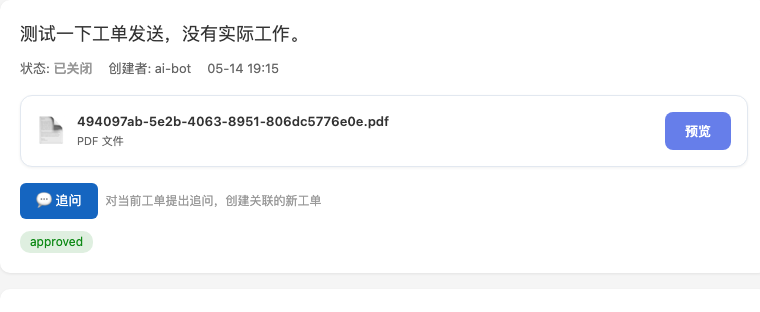
\includegraphics[width=0.78\textwidth]{screenshots/manual_fig1_detail.png}
\caption{工单详情页——「追问」按钮位于工单内容下方}
\label{fig:detail}
\end{figure}

\section{操作步骤}

\subsection{进入工单详情}

在工单列表页点击任意工单编号，进入详情页。
在工单内容下方可以看到 \textcolor{blue}{[追问] 追问} 按钮（\autoref{fig:detail} 中箭头所指），
该按钮对所有用户可见。

\subsection{点击「追问」}

点击 \textcolor{blue}{[追问] 追问} 按钮，系统自动跳转到新建工单页面，
并自动填写以下内容（\autoref{fig:create}）：

\begin{itemize}
  \item \textbf{标题}：自动填入 \texttt{追问 \#N: 原工单标题}
  \item \textbf{内容}：自动填入追问引用块
  \begin{itemize}
    \item \texttt{\#\# 追问自 \#N}
    \item \texttt{> 原工单 \#N: 原工单标题}
  \end{itemize}
\end{itemize}

\begin{figure}[h]
\centering
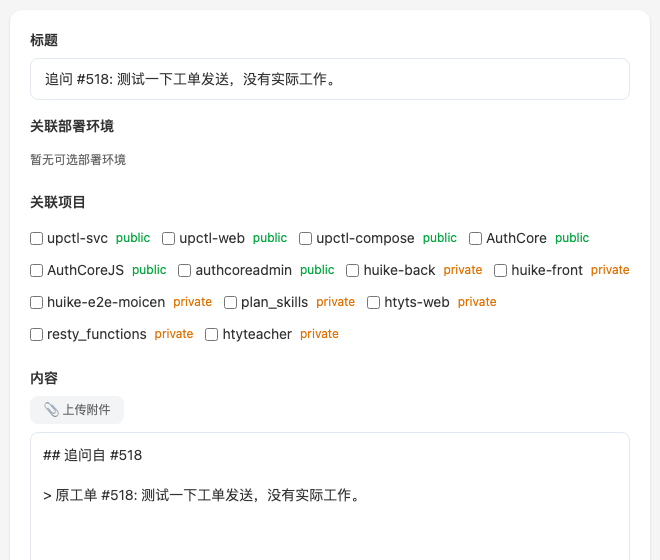
\includegraphics[width=0.82\textwidth]{screenshots/manual_fig2_create.png}
\caption{新建工单页面——标题和内容自动预填}
\label{fig:create}
\end{figure}

\subsection{填写追问内容}

在自动生成的引用内容下方（留有空行），输入您要追问的具体问题或补充信息。
支持 Markdown 格式，可以上传附件（图片、PDF、Word 文档等）。

\subsection{提交工单}

填写完成后点击「提交」按钮。新工单创建成功后会自动跳转到新工单详情页，
可以从标题中看到它是 \texttt{追问 \#N} 的关联工单。

\begin{figure}[h]
\centering
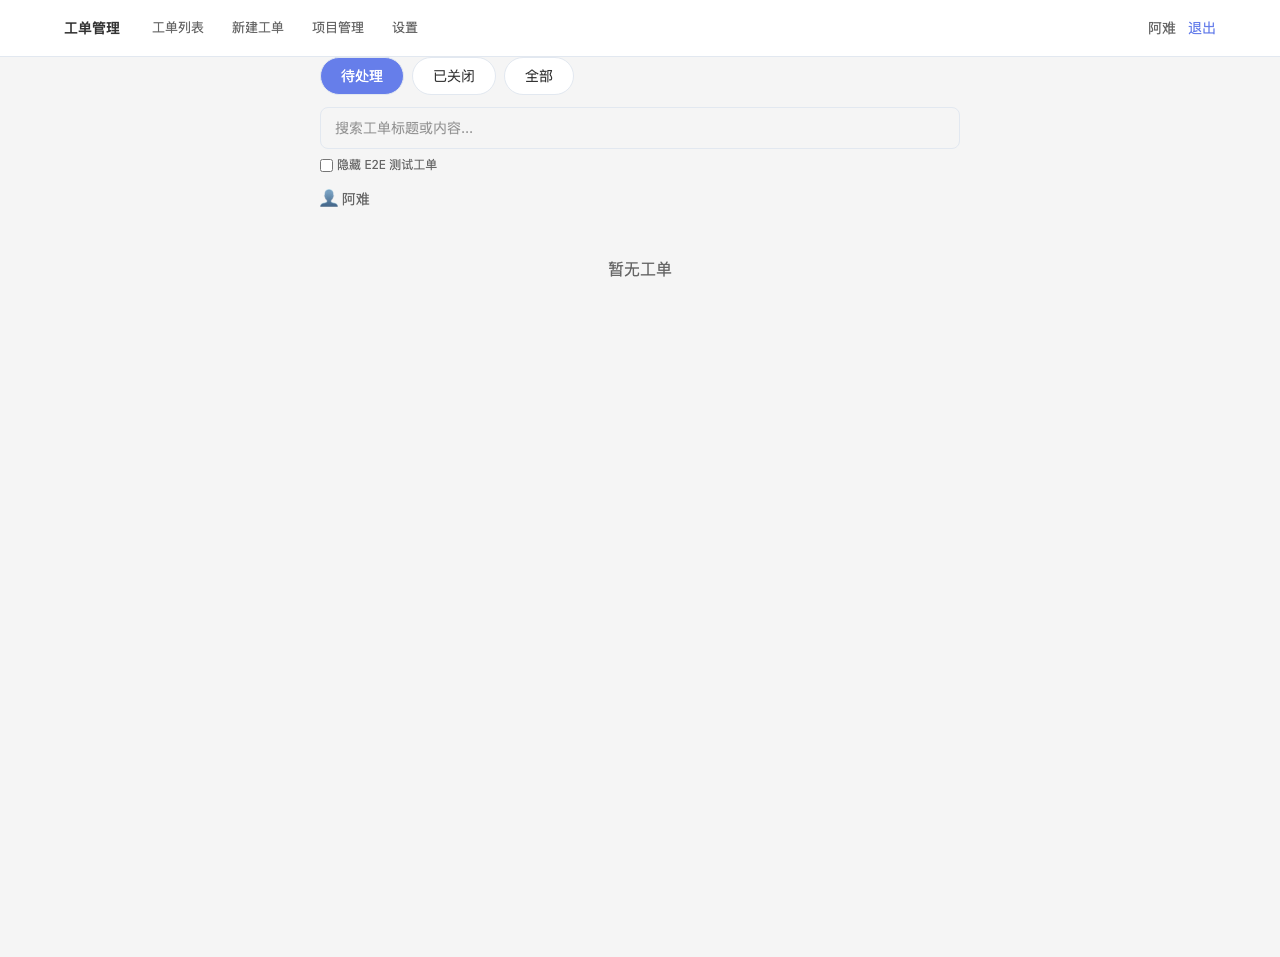
\includegraphics[width=0.82\textwidth]{screenshots/manual_fig3_list.png}
\caption{工单列表——追问生成的工单标题带有原工单编号}
\label{fig:list}
\end{figure}

\section{效果与追溯}

通过此功能可以实现：

\begin{itemize}
  \item \textbf{完整追溯}：追问工单的标题和内容都引用了原工单编号和标题，可以快速定位上下文
  \item \textbf{独立处理}：每个追问是一个独立工单，可以独立审批、分配和处理
  \item \textbf{持续迭代}：一个工单可以衍生多个追问，形成需求-追问-实现的完整链条
\end{itemize}

\section{注意事项}

\begin{itemize}
  \item 追问工单的标题会自动以 \texttt{追问 \#N:} 开头，强烈建议保留此前缀以便追溯
  \item 追问工单创建后与原工单独立，需要单独批准和处理
  \item 如需对追问再进行追问，重复上述步骤即可
\end{itemize}

\vfill
\begin{center}
\small \textcolor{gray}{—— 工单管理系统 ——}
\end{center}

\end{document}
